\documentclass{article}
\usepackage[utf8]{inputenc}
\usepackage[protrusion=true, expansion=true]{microtype}
\usepackage[hang, small, labelfont=bf, up, textfont=it, up]{caption}
\usepackage{listings}
\usepackage{ragged2e}
\usepackage{amsfonts}
\usepackage[font=small,labelfont=bf]{caption}

\usepackage{csvsimple} 
\usepackage{color}


\usepackage{algpseudocode}
\usepackage{algorithm}

\usepackage{changepage}

\usepackage{graphicx}
\usepackage{amsmath}
\usepackage{fancyhdr}
\usepackage[a4paper, total={7in, 10in}]{geometry}
\usepackage[ddmmyyyy]{datetime}
\usepackage{lipsum}

\usepackage{tikz}
\usepackage{tikz-qtree}
\usepackage{amsmath,bm,times}
\usetikzlibrary{shapes,arrows,calc,arrows.meta}
\usetikzlibrary{decorations.pathreplacing,positioning, calc,shapes.multipart,chains,arrows}
\tikzset{listnode/.style={rectangle split, rectangle split parts=2,
    draw, rectangle split horizontal}}
\tikzset{hashtable/.style={rectangle split, rectangle split parts=5,
    draw, rectangle split}}
 
\usetikzlibrary{positioning}

\tikzset{
node of list/.style = { 
             draw, 
             fill=blue!20, 
             minimum height=6mm, 
             minimum width=6mm,
             node distance=6mm
   },
link/.style = {
     -stealth,
     shorten >=1pt
     },
array element/.style = {
    draw, fill=white,
    minimum width = 6mm,
    minimum height = 10mm
  }
}
\tikzset{main node/.style={circle,fill=blue!20,draw,minimum size=1cm,inner sep=0pt},
            }
    
\newcommand{\mx}[1]{\mathbf{\bm{#1}}} % Matrix comman2
\newcommand{\vc}[1]{\mathbf{\bm{#1}}} % Vector command

% We need layers to draw the block diagram
\pgfdeclarelayer{background}
\pgfdeclarelayer{foreground}
\pgfsetlayers{background,main,foreground}
% Define a few styles and constants
\tikzstyle{sensor}=[draw, fill=blue!20, text width=5em, 
text centered, minimum height=3.5em]
\tikzstyle{ann} = [above, text width=6em]
\tikzstyle{naveqs} = [sensor, text width=6em, fill=red!20, minimum width=7em,
minimum height=8em, rounded corners]




%Opening
\title{Trabalho Prático 3 - Árvore de Segmentação}
\author{João Correia Costa (2019029027)}
\date{Dezembro de 2023, Belo Horizonte}

\begin{document}

\maketitle

\section{Introdução}

Árvores de Segmentação são estruturas de dados versáteis utilizadas em ciência da computação  para lidar eficientemente com várias tarefas de consulta de intervalo, em inglês, range-query. É particularmente útil em cenários nos quais você precisa realizar funções agregadas ou operações de atualização em um subvetor de elementos.

A ideia central por trás de uma árvore de segmentos é representar um vetor dado como uma árvore binária, onde cada nó folha corresponde a um elemento individual no vetor. Os nós internos da árvore armazenam informações agregadas (como a soma, mínimo, máximo, etc.) de seus respectivos nós filhos. Essa estrutura hierárquica permite consultas eficientes de intervalo e atualizações.

A construção de uma árvore de segmentos envolve a divisão recursiva do vetor em segmentos menores até que cada segmento represente um único elemento. Durante operações de consulta, a árvore é percorrida para encontrar os segmentos relevantes que contribuem para o resultado final, levando a soluções eficientes.

Essa abordagem é particularmente útil em cenários nos quais o vetor de entrada é estático, e a maioria das operações envolve consultas ou atualizações em intervalos específicos, pois oferece um equilíbrio entre complexidade de tempo e espaço.

No contexto mencionado, o presente trabalho busca implementar uma Árvore de Segmentação construída sobre um vetor de entrada que contém matrizes  \(A_{2 \times 2}\). Cada matriz representa uma transformação vetorial no espaço \(2D\), e um subvetor específico do vetor de entrada representa uma sequência de transformações vetoriais que pode ser sintetizada em uma única matriz \(R_{2 \times 2}\), resultante do produto de todas as matrizes no intervalo considerado. Em outras palavras, a transformação vetorial associada ao subvetor do índice \(i\) ao \(j\) é dada por \(A_i \times \ldots \times A_j = R_{ij}\). Neste sentido, os nós internos da árvore de segmentação contém matrizes resultantes  \(R_{ij}\) do produto de uma sequência de matrizes do segmento, e os nós folha contém matrizes simples, associada a uma transformação vetorial apenas.


Estamos buscando calcular a matriz de transformação  \(R_{ij}\)  associada a um determinado subvetor de matrizes, do índice \(i\) ao \(j\),  que será aplicada a um vetor 2D (cord\_x, cord\_y) fornecido. Essa matriz nos permitirá prever qual será o novo vetor resultante após a aplicação da transformação.


% Método
\section{Método}

A entrada de dados é composta por dois inteiros: $n$, que representa o tamanho do vetor de matrizes (ou seja, o número de matrizes de transformação), e $q$, indicando o número de operações a serem realizadas. Em seguida, as operações são descritas, uma por linha. Para consultas, é lido um caractere $q$ seguido por quatro inteiros $t_0$, $t_1$, $cord_x$, $cord_y$, indicando os índices do subvetor de matrizes a ser considerado na consulta e as coordenadas do ponto $(x, y)$ a ser transformado. Apenas os 8 dígitos menos significativos do ponto resultante após a transformação são impressos. Para operações de atualização, é lido um caractere $u$, seguido por um inteiro $a$, representando a posição no vetor de matrizes a ser alterada. As próximas linhas leem uma matriz 2D que deve substituir a matriz na posição $a$ do vetor. A operação de atualização não possui nenhuma saída esperada.

Duas soluções foram implementadas. A primeira consiste em armazenar cada uma das transformações em um arranjo indexado.  A segunda estratégia envolve a implementação de uma Árvore de Segmentação que armazena matrizes de transformação pré-computadas em seus nós.


\subsection{Vetor Simples de Matrizes}

Uma abordagem simplificada para o problema seria armazenar cada uma das transformações em um vetor indexado de matrizes. Para a operação de consulta, considerando os instantes (índices) $i$ e $j$, seria suficiente multiplicar todas as matrizes nos índices de $i$ a $j$. No pior caso, essa abordagem tem complexidade $O(n)$. Para as operações de atualização, bastaria modificar a matriz na posição $i$, o que é feito em tempo constante. Ver Figura 1.


\subsection{Árvore de Segmentação}

A segunda abordagem adotada para resolver o problema consiste na implementação de uma Árvore de Segmentação que armazena matrizes de transformação pré-computadas em seus nós. Essa estratégia tem como objetivo otimizar a execução das operações de consulta de maneira eficiente.

\subsubsection{Construção da Árvore}

A construção da Árvore de Segmentação é um processo realizado de maneira recursiva, onde cada nó interno da árvore representa um intervalo do vetor de matrizes. O método utilizado para implementar essa construção é denominado \texttt{SegTree::build}.

No início do processo, a raiz da árvore é configurada para representar o intervalo completo do vetor de matrizes. Cada nó interno da árvore armazena o produto das matrizes dentro do intervalo correspondente. A construção ocorre de forma recursiva até que cada nó folha contenha uma única matriz de transformação.

No código fornecido, a função \texttt{SegTree::build} recebe quatro parâmetros: o índice do nó atual $p$, os limites esquerdo e direito do intervalo $l$ e $r$, e um ponteiro para um array de matrizes \texttt{array}.

A construção da árvore é realizada da seguinte maneira:

\begin{itemize}
    \item Se o intervalo $l$ é igual a $r$, ou seja, estamos em um nó folha, a função retorna a matriz correspondente a esse índice no array.
    \item Caso contrário, calcula-se o ponto médio $m$ do intervalo e continua a construção para os filhos esquerdo e direito de forma recursiva.
    \item As matrizes obtidas dos filhos são multiplicadas para obter a matriz resultante representando o intervalo atual.
    \item A matriz anteriormente armazenada no nó atual é liberada, e o nó atual é atualizado com a nova matriz resultante.
\end{itemize}

Essa abordagem garante que a árvore seja construída de forma eficiente, armazenando produtos de matrizes nos nós internos e mantendo a consistência ao longo da estrutura da árvore.


\subsubsection{Consulta na Árvore}

Na etapa de consulta na Árvore de Segmentação de Matrizes, o procedimento segue uma lógica sequencial.Ao iniciar a consulta, verifica-se se o nó atual na árvore possui alguma interseção com o intervalo desejado. Se não houver interseção, a matriz identidade é retornada como resultado, indicando que não é necessário continuar a exploração nesse ramo específico da árvore.

Em seguida, examina-se se o nó atual está completamente contido no intervalo da consulta. Caso afirmativo, a matriz armazenada nesse nó é retornada integralmente como resultado, eliminando a necessidade de buscar mais informações nesse ramo da árvore.

Se o nó atual apresentar apenas uma interseção parcial com o intervalo da consulta, o processo se ramifica. A consulta é repetida para o filho esquerdo e para o filho direito do nó atual. As respostas obtidas desses filhos são então combinadas multiplicando as matrizes correspondentes.

Por fim, a resposta final é representada pela matriz resultante da combinação das respostas dos filhos. Dessa maneira, a consulta na Árvore de Segmentação de Matrizes é conduzida de forma eficiente, explorando apenas os ramos relevantes e utilizando a matriz identidade como um elemento neutro para casos específicos. A consulta na árvore foi implementada no método \texttt{SegTree::query}.

\subsubsection{Atualização na Árvore}

Na etapa de atualização na Árvore de Segmentação de Matrizes, o processo inicia-se pela localização do nó correspondente à posição $a$ no vetor de matrizes. Esse nó é identificado para representar a matriz que será atualizada. Posteriormente, realiza-se a substituição da matriz armazenada nesse nó pela nova matriz fornecida como entrada, efetuando a atualização na posição específica do vetor de matrizes.

O próximo passo envolve uma propagação recursiva em direção aos nós pais. Em cada nó pai ao longo do caminho até a raiz da árvore, recalcula-se a matriz armazenada no nó pai com base nas novas matrizes dos filhos. Essa propagação recursiva é executada até alcançar a raiz da árvore, assegurando a consistência das matrizes nos nós pais.

Dessa forma, a operação de atualização garante a substituição adequada da matriz na posição $a$ do vetor e mantém a integridade da representação das transformações ao longo da estrutura da árvore. A atualização na árvore foi implementada no método \texttt{SegTree::update}.


Com essa implementação, busca-se melhorar o desempenho, especialmente em cenários nos quais as operações de consulta são frequentes em comparação com as operações de atualização.


\begin{figure}
  \centering

  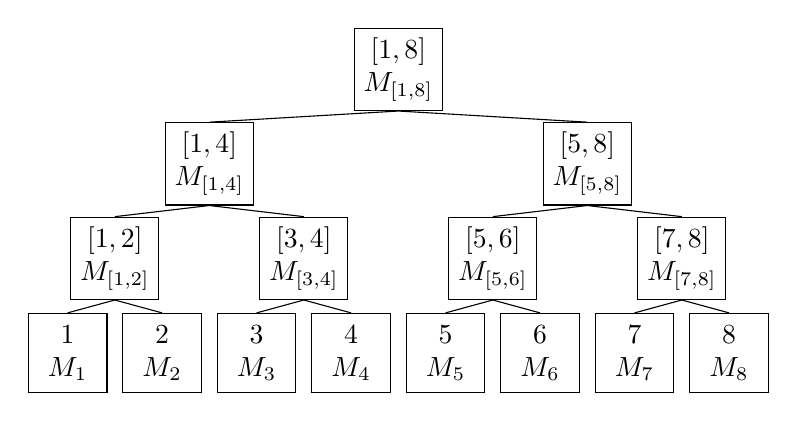
\begin{tikzpicture}[scale=0.8,level distance=1.5cm,
    level 1/.style={sibling distance=6cm},
    level 2/.style={sibling distance=3cm},
    level 3/.style={sibling distance=1.5cm},
    every node/.style={draw, rectangle, minimum size=1cm, align=center}]
    
    \node {$[1, 8]$ \\ $M_{[1,8]}$}
      child {node {$[1, 4]$ \\ $M_{[1,4]}$}
        child {node {$[1, 2]$ \\ $M_{[1,2]}$}
          child {node {$1$ \\ $M_{1}$}}
          child {node {$2$ \\ $M_{2}$}}}
        child {node {$[3, 4]$ \\ $M_{[3,4]}$}
          child {node {$3$ \\ $M_{3}$}}
          child {node {$4$ \\ $M_{4}$}}}}
      child {node {$[5, 8]$ \\ $M_{[5,8]}$}
        child {node {$[5, 6]$ \\ $M_{[5,6]}$}
          child {node {$5$ \\ $M_{5}$}}
          child {node {$6$ \\ $M_{6}$}}}
        child {node {$[7, 8]$ \\ $M_{[7,8]}$}
          child {node {$7$ \\ $M_{7}$}}
          child {node {$8$ \\ $M_{8}$}}}};
  \end{tikzpicture}
  \quad
  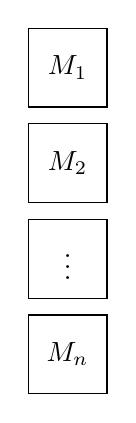
\begin{tikzpicture}[scale=0.8, every node/.style={draw, rectangle, minimum size=1cm, align=center}]
    \node {$M_1$};
    \node[below=0.2cm of current bounding box.south, anchor=north] {$M_2$};
    \node[below=0.2cm of current bounding box.south, anchor=north] {$\vdots$};
    \node[below=0.2cm of current bounding box.south, anchor=north] {$M_n$};
  \end{tikzpicture}

  \vspace{1em} % Espaço entre as duas figuras


  \caption{Árvore de Segmentação à esquerda e Vetor Ingênuo à direita.}
\end{figure}



\section{Análise de Complexidade}
Essa seção se dedica a analisar a complexidade assintótica, em termos de espaço e de tempo, das funções de consulta, atualização e construção na árvore de segmentação e no vetor simples de matrizes.

\subsection{\texttt{SegTree::build}}
\begin{itemize}
    \item A operação de construção da árvore de segmentação (\texttt{SegTree::build}) pode ser convenientemente descrita de forma recursiva, percorrendo a árvore a partir do vértice raiz até os vértices folha.
    \item O procedimento de construção, quando chamado em um vértice não folha, realiza o seguinte:
        \begin{enumerate}
            \item Constrói recursivamente as matrizes dos dois vértices filhos.
            \item Multiplica a matriz dos vértices filhos para obter a matriz do nó.
        \end{enumerate}
    \item O início da construção ocorre no vértice raiz, permitindo a computação da árvore de segmentação completa.
    \item A complexidade de tempo dessa construção é \(O(n)\), considerando que a operação de multiplicação (\texttt{Matrix* operator*(const Matrix\& other)}) é de tempo constante (a operação de multiplicação é chamada \(n\) vezes, que é igual ao número de nós internos na árvore de segmentação).
\end{itemize}


\subsection{\texttt{SegTree::query}}
A consulta opera dividindo o segmento de entrada em vários subsegmentos, para os quais todas as matrizes já foram previamente calculadas e armazenadas na árvore. A eficiência característica da Árvore de Segmentação consiste na possibilidade de interromper a consulta no ramo sempre que o nó coincide com o range de busca ou está contido nele. No pior caso temos custo  \(O(\log n)\), onde n é o número de nós na árvore.


\subsection{\texttt{SegTree::update}}

Quando desejamos modificar um elemento específico no vetor, por exemplo, realizar a atribuição \(vetor[i] = M\), é necessário reconstruir a Árvore de Segmentação de modo a corresponder ao novo array modificado. Todo o ramo associado ao índice $i$ é afetado, então caminhamos da folha até a raiz recalculando as matrizes nos nós, temos custo  \(O(\log n)\).

\subsection{\texttt{SimpleVector::build}}
Aloca-se espaço para o vetor e percorre cara índice sequenciamente adicionando uma matriz identidade, tem-se custo linear \(O(n)\).

\subsection{\texttt{SimpleVector::update}}
Apenas deletamos a matriz no índice $i$ de atualização e substituímos por uma nova matriz. Temos custo constante  \(O(1)\).

\subsection{\texttt{SimpleVector::query}}
Varremos o vetor sequencialmente entre os índices de busca $i$ e $j$, multiplicando as matrizes e armazenando em uma matriz resultante, tem-se custo  \(O(n)\).

\subsection{\texttt{SimpleVector::build}}
Varremos o vetor sequencialmente entre os índices de busca $i$ e $j$, multiplicando as matrizes e armazenando em uma matriz resultante, tem-se custo  \(O(n)\).

   


% Estratégias de Robustez

\section{Estratégias de Robustez}
Com o objetivo de tornar o programa mais robusto e evitar problemas com entradas inválidas, foram criadas classes de exceção \texttt{ExceptionEmptyList}. Essa exceção é disparada, com uma mensagem de erro descritiva, caso a função de remoção de um elemento da lista seja invocada para uma estrutura vazia. 

Para manter a integridade do programa e evitar vazamentos de memória, todos os Tipos Abstratos de Dados (TADs) implementam destrutores apropriados. Nos destrutores da lista encadeada, garantimos que o estado da instância retorne ao \texttt{default} e \texttt{asserts} checam se o tamanho da estrutura é zero.

Além disso, foram realizados testes com o Valgrind, e nenhum erro relacionado à alocação de memória foi observado.

Entretanto, é importante destacar que o programa ainda possui limitações, uma vez que não cobre um amplo espectro de possíveis entradas de dados, presumindo que o usuário fornecerá entradas corretas. 


\section{Análise Experimental}

\subsection{Algoritmos de Ordenação}
O presente experimento foi conduzido com o propósito de avaliar o custo computacional de diferentes algoritmos de ordenação. Foram gerados 29 grafos, variando o número de vértices de 1000 a 30000. A quantidade de arestas em cada grafo foi estabelecida como 50\% superior ao número de vértices. O tempo de execução de cada algoritmo de ordenação foi medido em relação a esses grafos, utilizando a biblioteca \texttt{chrono}. Os resultados temporais obtidos foram então representados graficamente, conforme ilustrado na Figura no Apêndice B.



Ao analisar o gráfico, destacam-se três grupos de desempenho. O grupo de pior desempenho inclui os algoritmos \texttt{bubble\_sort} e \texttt{selection\_sort}; em segundo lugar, temos o \texttt{insertion\_sort}; e o terceiro grupo engloba os demais algoritmos, que apresentam um custo temporal abaixo de décimos de segundo para todos os grafos.

Presume-se que o desempenho superior do \texttt{insertion\_sort} em relação ao primeiro grupo deve-se à sua adaptabilidade a dados parcialmente ordenados, ou seja, os grafos fornecidos já possuem uma ordenação razoável. Os algoritmos do primeiro grupo não se beneficiam da ordenação parcial.

Como esperado, os algoritmos \texttt{merge\_sort}, \texttt{heap\_sort}, \texttt{quick\_sort} apresentaram desempenho muito superior aos outros grupos, especialmente para grafos grandes. Isso pode ser explicado, em primeiro lugar, pela função de complexidade desses três algoritmos, que no pior caso é \(O(n \log n)\) para o \texttt{merge\_sort} e \texttt{heap\_sort}, e \(O(n^2)\) para o \texttt{quick\_sort}, embora geralmente o \texttt{quick\_sort} apresente \(O(n \log n)\), conforme observado no gráfico.

Além disso, o uso de estruturas de dados auxiliares, como Heaps e arrays extras, também contribuem para a eficiência desses três algoritmos.

No grupo de melhor desempenho, é destacado um terceiro algoritmo de ordenação: o Count Sort. O Count Sort é eficiente para conjuntos de dados com um intervalo pequeno de valores, como é o caso dos grafos do experimento, que têm uma faixa limitada de cores. Sua complexidade temporal é linear \(O(n)\), onde \(n\) é o número de vértices, o que o torna uma escolha eficiente para o problema proposto.


\subsection{Validação}

Ao analisarmos o tempo de execução da função de validação da coloração dos grafos, observamos uma curva linear, o que está em conformidade com a análise de complexidade \(O(n)\). A Figura correspondente pode ser encontrada no Apêndice B.
Essa análise é fundamentada na compreensão da complexidade dos métodos envolvidos na validação da coloração: \texttt{bool validate\_grapgh} e \texttt{bool validate}.




\section{Conclusões}

No projeto, abordamos o problema clássico de coloração em grafos, com ênfase na complexidade algorítmica e nas estruturas de dados implementadas em C++. Inicialmente, desenvolvemos um algoritmo para identificar se a coloração do grafo é gulosa, isto é, se um vértice \(v\) possui coloração \(i\), então ele possui pelo menos um vizinho com cada uma das cores menores que \(i\). Em seguida, aplicamos algoritmos clássicos de ordenação, seguindo o critério de cor e índice, conforme descrito na função \texttt{bool criterium}.

Ao longo do projeto, aprofundamos nosso entendimento das estruturas de dados eficientes para modelagem de grafos, como a combinação de array e lista encadeada. Também exploramos os algoritmos de ordenação clássicos, destacando as nuances entre suas complexidades assintóticas em termos de tempo e memória.

Este trabalho não apenas ampliou nossa habilidade de implementar soluções algorítmicas em C++, mas também proporcionou insights sobre a escolha e aplicação de estruturas de dados e algoritmos em cenários específicos, contribuindo para uma compreensão mais abrangente da ciência da computação.





\section{Bibliografia}
1. Chaimowicz, L. and Prates, R. (2020). Slides virtuais da disciplina de estruturas de dados. Disponibilizado via moodle. Departamento de Ciência da Computação. Universidade
Federal de Minas Gerais. Belo Horizonte. 
\justify
2. Introduction to Algorithms, Thomas H. Cormem, Charles E. Leiserson, Ronald L. Rivest.




\appendix
\newpage
\section{Instruções para Compilação e Execução}
\label{ap:compilacao_execucao}

\textbf{Observação:} Certifique-se de que você tenha o compilador GCC (g++) instalado em seu sistema para a compilação.

\subsection{Compilação do Projeto}

Para compilar o projeto, siga as instruções abaixo:

\begin{enumerate}
    \item Abra um terminal e navegue até o diretório raiz do projeto.
    \item Certifique-se de que o projeto contenha a seguinte estrutura de diretórios:
    
    \begin{verbatim}
    - src/
    - obj/
    - bin/
    - include/
    \end{verbatim}

    \item Utilize o seguinte comando para compilar o projeto:

    \begin{verbatim}
    make ou make all
    \end{verbatim}

    Isso irá compilar o projeto e gerar o executável \texttt{bin/tp2.out}.

\end{enumerate}

\subsection{Execução do Projeto}

Para executar o projeto compilado, utilize o seguinte comando:

\begin{verbatim}
./bin/tp2.out
\end{verbatim}

Este comando executará o programa principal.


\subsection{Limpeza dos Arquivos Compilados}

Para limpar os arquivos compilados e executáveis, utilize o seguinte comando:

\begin{verbatim}
make clean
\end{verbatim}

Isso removerá os arquivos objetos e executáveis.

\newpage
\section{Figuras}

\begin{figure}[H]
    \begin{minipage}{\textwidth}
        \centering
        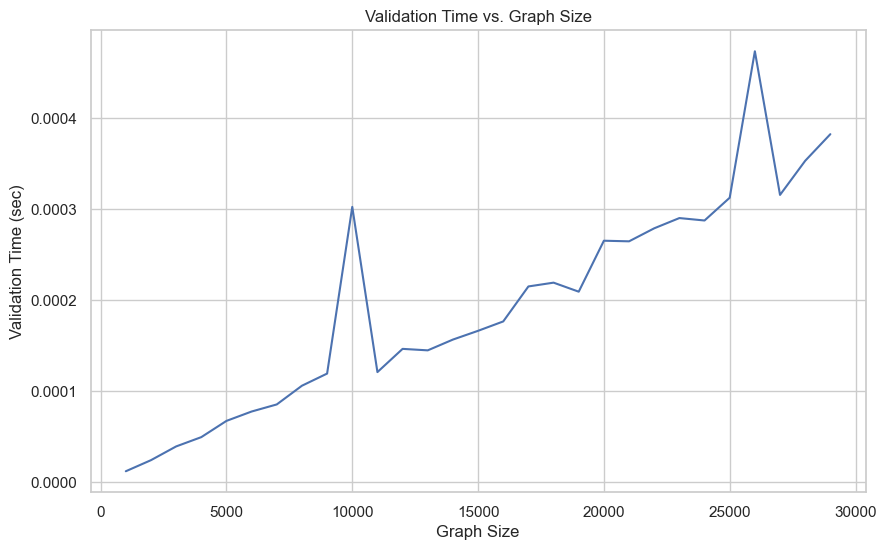
\includegraphics[width=0.8\linewidth]{~/Documents/UFMG-CODE/graphColoration/experiments/validation_time_vs_graph_size.png}
        \caption{Desempenho da função de validação dos grafos do experimento.}
        \label{fig:validacao}
    \end{minipage}
\end{figure}

\vspace{1cm}

\begin{figure}[H]
    \begin{minipage}{\textwidth}
        \centering
        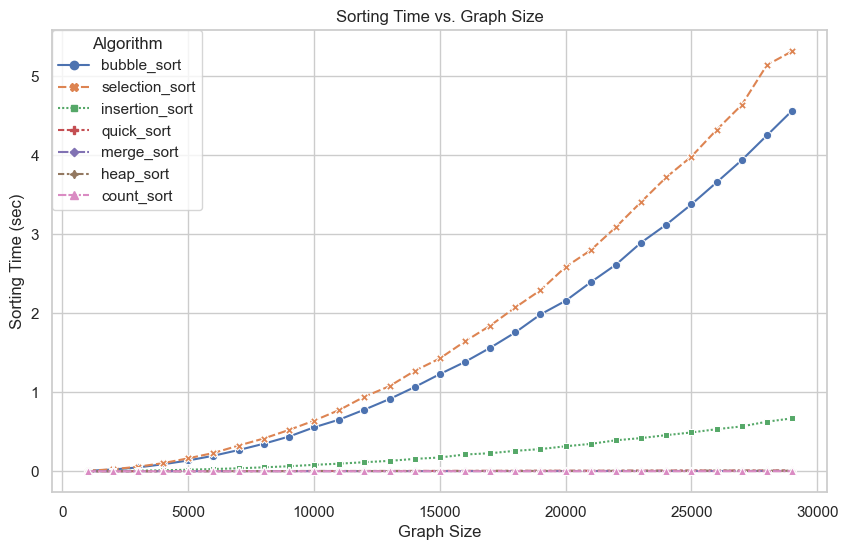
\includegraphics[width=0.8\linewidth]{~/Documents/UFMG-CODE/graphColoration/experiments/sorting_time_vs_graph_size.png}
        \caption{Desempenho dos algoritmos de ordenação para os grafos do experimento.}
        \label{fig:ordenacao}
    \end{minipage}
\end{figure}

\label{ap:figuras}


\end{document}
